%\documentclass{article}
\documentclass{llncs}

% NETYS requirements
%  15 pages in Springer’s LNCS format, excluding bibliographic references,

\usepackage{floatpag}
\floatpagestyle{empty} 

\usepackage{graphicx} % Required for inserting images
\usepackage[ruled,vlined,linesnumbered]{algorithm2e}
\usepackage{comment}
%\usepackage{enumitem}

\newtheorem{assumption}{Assumption}
\newtheorem{deliverycondition}{Delivery Condition}

\usepackage[hidelinks]{hyperref}
\def\assumptionautorefname{Assumption}
\def\propositionautorefname{Proposition}
\def\lemmaautorefname{Lemma}
\def\theoremautorefname{Theorem}
\def\corollaryautorefname{Corollary}
\def\deliveryconditionautorefname{Delivery Condition}

% no newline after subsection header
\let\llncssubparagraph\subparagraph
\let\subparagraph\paragraph
\usepackage{titlesec}
\let\subparagraph\llncssubparagraph
\titleformat{\subsection}[runin]
    {\normalfont\bfseries}{}{0em}{}[.]

\usepackage{tikz}

\usepackage{amsmath}

\def\Byz{f}   % the Byzantine node
\def\ByzN{x}  % number of Byzantine nodes
\def\L{\mathsf{L}}  % left-hand-rule
\def\R{\mathsf{R}}  % right-hand-rule


% make definitions italic instead of bold
%\setlist[description]{font=\normalfont\itshape}

% NETYS requirements
%  15 pages in Springer’s LNCS format, excluding bibliographic references,


\title{BeRGeR Bloopers}
\subtitle{Material not included in the paper}
\author{Brown Zaz}
\institute{Department of Computer Science, Kent State University, Kent, OH 44242, USA\\
\email{zbrown@cs.kent.edu}}
\date{}

\begin{document}

\maketitle
\thispagestyle{plain}
\pagestyle{plain}


% +~~~~~~~~~~~~~~~~~~~~~~~~~~~~~~~~~~~~~~~~~~~~~~~~~~~~~~~~~~~~~~~~~~~~~~~~~~~~~~~~~~~~~~~~~~~~~~~~~~~~~~~~~~+ %
% | TODO:  MN, see the email sent 3/13                                                                       | %
% |        We may want to keep this part as separate and accessible as possible to a wider audience.         | %
% |        Collective disjointness possibly has applications to transport networks that require redundancy.  | %
% +~~~~~~~~~~~~~~~~~~~~~~~~~~~~~~~~~~~~~~~~~~~~~~~~~~~~~~~~~~~~~~~~~~~~~~~~~~~~~~~~~~~~~~~~~~~~~~~~~~~~~~~~~~+ %
\subsection{Redundant routing}
% TODO: cite who? Dolev?
Without cryptography, deterministically delivering a message from \(s\) to \(t\) requires that either \(s\) and \(t\) are neighbors (the trivial case which, for the purposes of this paper, we ignore) or that there exist \(2\ByzN + 1\) disjoint paths between \(s\) and \(t\). This means for any deterministic Byzantine-resistant routing algorithm to work for all pairs of nodes, there must be \(2\ByzN + 1\) disjoint paths between each pair of nodes in the network. By Menger's theorem, this is equivalent to requiring the network be \((2\ByzN + 1)\)-connected.

In spite of the necessity of \(2\ByzN + 1\) disjoint paths, the key insight to this routing algorithm is that packets do need to traverse these disjoint paths. If you have more than \(2\ByzN + 1\) packets, it is not necessary that the paths they take be pairwise disjoint; the more general condition that they are \emph{collectively disjoint} is sufficient. Intuitively, this means that the union of the paths traversed by the nodes must contain \(2\ByzN + 1\) disjoint paths, but the packets do not need to follow those disjoint paths. The paths the packets take may overlap. When the paths overlap, but collective disjointness is maintained, this is called \emph{braiding}.

It is easier to find collectively disjoint paths than pairwise disjoint paths because collective disjointness (CD) is less restrictive than pairwise disjointness (PD), as can be seen from their respective termination conditions:
\begin{align*}
    \exists i, j\phantom{, k, ...} \ &: \ m_i = m_j, \phantom{ = m_k = \cdots,} \ p_i \cap p_j \phantom{\cap p_k \cap \cdots} \ = \emptyset \tag{PD} \\
    \exists i, j         , k, ...  \ &: \ m_i = m_j            = m_k = \cdots,  \ p_i \cap p_j          \cap p_k \cap \cdots  = \emptyset \tag{CD}
\end{align*}


\section{Tikz diagrams}

% thicker lines
\tikzset{every picture/.style={line width=.8pt}}
\def\myNode[#1](#2) {
    %\filldraw[white,draw=black] (#2) circle (7pt) node[scale=1.5,anchor=center,black]{#1};  % circled letters
    \filldraw[black,draw=white,line width=3pt] (#2) circle (3pt) node[scale=1.5,anchor=west,black]{\(#1\)};  % dots with space around them
}
\def\stLine(#1)(#2) {
    \draw[gray, dashed] (#1) -- (#2);  % s-t
}

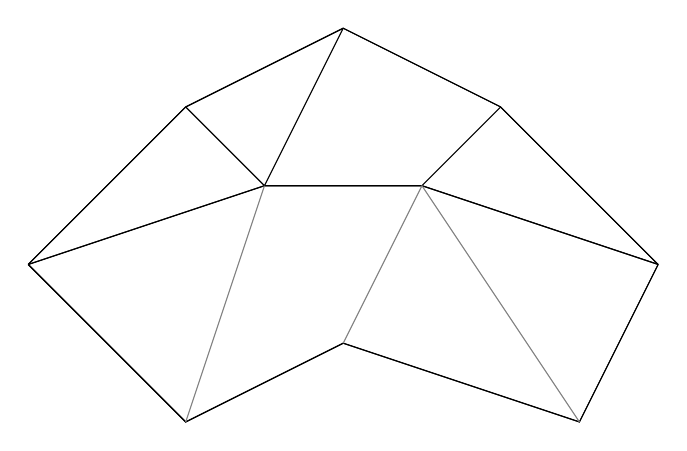
\begin{tikzpicture}
    \stLine(0,0)(8,0)

    \draw (0, 0) -- (2, 2) -- (4, 3) -- (6, 2) -- (8,0);  % s-a-d-g-t
    \draw (0, 0) -- (3, 1) -- (5, 1)           -- (8,0);  % s-b-e-t
    \draw (0, 0) -- (2,-2) -- (4,-1) -- (7,-2) -- (8,0);  % s-c-f-i-t

    \draw[smooth] (0, 0) -- (2, 2) -- (4, 3) -- (6, 2) -- (8,0);  % s-a-d-g-t
    \draw[smooth] (0, 0) -- (3, 1) -- (5, 1)           -- (8,0);  % s-b-e-t
    \draw[smooth] (0, 0) -- (2,-2) -- (4,-1) -- (7,-2) -- (8,0);  % s-c-f-i-t

    \draw (2, 2) -- (3, 1) -- (4, 3);  % a-b-d
    \draw (5, 1) -- (6, 2);  % e-g

    \draw[gray] (3,1) -- (2,-2);  % b-c
    \draw[gray] (5,1) -- (4,-1);  % e-f
    \draw[gray] (5,1) -- (7,-2);  % e-i

    \myNode[s](0, 0)

    \myNode[a](2, 2)
    \myNode[b](3, 1)
    \myNode[c](2,-2)

    \myNode[d](4, 3)
    \myNode[e](5, 1)
    \myNode[f](4,-1)
    
    \myNode[g](6, 2)
    \myNode[i](7,-2)

    \myNode[t](8,0)
\end{tikzpicture}


\begin{figure}[ht]
\centering
\begin{tikzpicture}
    \stLine(0,0)(8,0)

    \draw (0, 0) -- (2, 2) -- (4, 3) -- (6, 2) -- (8,0);  % s-a-d-g-t
    %\draw[lightgray] (0, 0) -- (3, 1) -- (5, 1);          % s-b-e
    \draw                     (5, 1)           -- (8,0);  %     e-t
    \draw (0, 0) -- (3,-2) -- (5,-1) -- (7,-2) -- (8,0);  % s-c-f-i-t

    %\draw[lightgray] (2, 2) -- (3, 1) -- (4, 3);  % a-b-d
    \draw (5, 1) -- (6, 2);  % e-g

    %\draw[lightgray] (3,1) -- (3,-2);  % b-c
    %\draw[lightgray] (5,1) -- (5,-1);  % e-f
    %\draw[lightgray] (5,1) -- (7,-2);  % e-i

    \myNode[s](0, 0)

    \myNode[a](2, 2)
    \myNode[b](3, 1)
    \myNode[c](3,-2)

    \myNode[d](4, 3)
    \myNode[e](5, 1)
    \myNode[f](5,-1)
    
    \myNode[g](6, 2)
    \myNode[i](7,-2)

    \myNode[t](8,0)
\end{tikzpicture}
\caption{Skipping b}
\end{figure}



\begin{tikzpicture}
    \stLine(-5,0)(5,0)

    \draw (-5,0) -- (-2,3);  % s-a
    \draw (-5,0) -- (-2,2);  % s-b
    \draw (-5,0) -- (-2,1);  % s-c
    
    \draw (-2,3) -- (-2,1);  % a-c
    
    \draw[gray] (-2,3) -- (2,-1);  % a-d
    \draw[gray] (-2,2) -- (2,-2);  % b-e
    \draw[gray] (-2,1) -- (2,-3);  % c-f
    
    \draw (2,-1) -- (2,-3);  % d-f
    
    \draw  (5,0) -- (2,-1);  % d-t
    \draw  (5,0) -- (2,-2);  % e-t
    \draw  (5,0) -- (2,-3);  % f-t

    \myNode[s](-5,0)

    \myNode[a](-2,3)
    \myNode[b](-2,2)
    \myNode[c](-2,1)

    \myNode[d](2,-1)
    \myNode[e](2,-2)
    \myNode[f](2,-3)

    \myNode[t](5,0)
\end{tikzpicture}


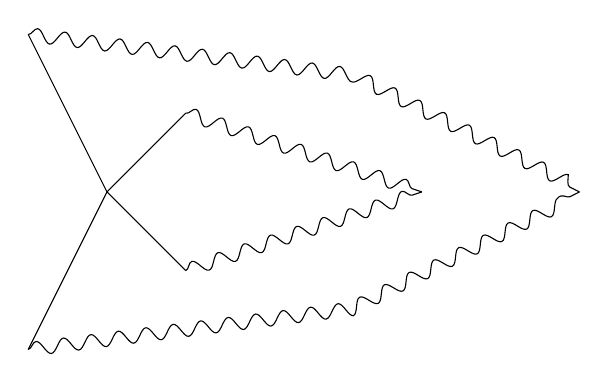
\begin{tikzpicture}    
\usetikzlibrary{decorations.pathmorphing}

\tikzset{snake it/.style={decorate, decoration=snake}}
    \stLine(4,0)(6,0) % s-t

    \draw (0,0) -- (-1, 2);  % n-o
    \draw (0,0) -- (-1,-2);  % s-p
    \draw (0,0) -- ( 1, 1);  % n-l
    \draw (0,0) -- ( 1,-1);  % n-m

    % TODO: MN: Why do we have [dotted] here? -Zaz
    \draw[snake it, smooth] (1, 1) -- (4,0);  % a-s
    \draw[snake it, smooth] (1,-1) -- (4,0);  % b-s

    \draw[snake it, smooth, tension=1] (-1, 2) -- (3,1.5) -- (6,0);  % c-t
    \draw[snake it, smooth] (-1,-2) -- (3,-1.5) -- (6,0);  % d-t

    \myNode[s](4,0)

    \myNode[x](0,0)

    \myNode[a](1,1)
    \myNode[b](1,-1)
    
    \myNode[c](-1,2)
    \myNode[d](-1,-2)

    \myNode[t](6,0)
\end{tikzpicture}

\newpage

\section{Old Pseudocode}

\begin{algorithm}[htb]

\footnotesize
\caption{BeRGeR variables and  functions}\label{algBERGERfunctions}
\SetKwProg{nextNode}{nextNode\((p, s, t, c, k)\)}{}{}
\SetKwProg{onThisSideOf}{onThisSide\((s, t, n, i)\)}{}{}
\SetKwFunction{onThisSide}{onThisSide}
\SetKw{and}{\ and\ }
\SetKwData{R}{R}
\SetKwData{L}{L}

\textbf{functions}\\
\vspace{1mm}
\nextNode(){}{

    \(\mathbf{loop\ for}\) \(i \in N\) starting with \(p\) in direction \(c \in \{\L, \R\} \) \\
        \ \ \ \ \ \ \If{\( i \neq k \and \onThisSide(s, t, n, i) \)}{
            \ \ \ \ \ \ \textbf{return} \( i \)
        }
    \textbf{return} \( \bot \)  \tcp*[f]{no next node found} \\

}


\end{algorithm}


\newpage

\section{Old Introduction}

We have a network (graph), \(G\), of nodes that know only the current packet, their position, and the set of their neighbors' positions.  They do not have space for routing tables, nor space to store information about packets that pass through them.  The goal is to route a message from \(s\) to \(t\) such that \(t\) will decode the correct message even in the presence of 1 node that behaves arbitrarily (i.e. is Byzantine).


The simplest solution without a Byzantine node would be to greedy route; at each step going to the node geometrically closest to \(t\). However, local minima result in this naïve algorithm not reaching \(t\). A guaranteed solution is to include draw a line through \(s\) and \(t\) (encoded in the packet), and then route along all edges of any face that intersects the \(s-t\) line. This was done in Concurrent Face Routing ~\cite{CFR} and is adapted here to generate 2 disjoint paths, or ``cores'', that form the core of our braided routing algorithm.

The state of the art in Geometric routing is GOAFR+ ~\cite{KuhnWattenhofer} where they route packets within an ellipse, increasing the size of the ellipse if progress is not made. They demonstrate practical efficiency and prove their algorithm is asymptotically optimal in the worst-case: \(O(p^2)\), where \(p\) is the shortest path length from \(s\) to \(t\), and assuming a unit-disk graph (UDG). We attempted something similar, but were stymied by networks where the external face intersected the \(s-t\) line in multiple places; we may attempt this again assuming no such intersections.

% gokarna: wondering whether this para is needed. May be need to define waht ICCs are and how are they related to our problem?
Finally, ~\cite{ICCs-ECCs} proves a correspondence between interactive consensus conditions (ICCs) and error-correcting codes (ECCs).  But I believe the ICCs apply to broadcast networks (complete graphs), so are not directly applicable here.

\newpage

\section{Definitions}

\begin{description}
  \item[ proximal sender ] the node the current packet was received from
  \item[ \(\overline{st}\) ] the line segment between \(s\) and \(t\)
  \item[ \(G\) ] the graph
  \item[ \(G-\overline{st}\) ] the graph with edges that intersect \(\overline{st}\) removed
  %\item[ green face ] a face that intersects \(\overline{st}\)
  \item[ superface ] the union of faces that intersect \(\overline{st}\)
  \item[ green node ] a node adjacent to the superface. This includes \(s\) and \(t\).
  \item[ core ] a packet that traverses the superface using either right-hand-rule (R) or left-hand-rule (L)
  \item[ braid ] a packet that is routed exactly as a core packet, except it skips a single node, \(k\), indicated in the packet
  \item[ braid chain ] a set of braids that collectively skip each node a core packet visited
  \item[ matching packets ] packets that contain the same \(m, s, t\)
\end{description}
% I don't believe these are necessary. We can simply refer to the neighboring faces of g
%\emph{\(g\)-purple face} - a union of non-green faces adjacent to a certain green node \(g\). \\

There are two kinds of packets: Cores and braids. Both packets contain:
\begin{description}
  \item[ \(m\) ] the message, comparable for equality
  \item[ \(s\) ] the ultimate source of the message
  \item[ \(t\) ] the ultimate target of the message
  \item[ \(c\) ] the chirality of the packet: R or L
\end{description}

\noindent
In addition, cores contain:
\begin{description}
  \item[ \(\ell\) ] the set of nodes the packet has visited
\end{description}

\noindent
And braids contain:
\begin{description}
  \item[ \(k\) ] the node the packet should block/skip
\end{description}

So cores have size proportional to the core path length, while braids are constant size (\(\log n\) bits). The fact that packets contain chirality means that when a packet arrives at a node, it is not only associated with an edge, but also a face.


\begin{deliverycondition}\label{dc:cores}
Target receives matching core R and L packets
\end{deliverycondition}
\begin{deliverycondition}\label{dc:braids}
Target receives a core and matching braids that skip each node in \(\ell\)
\end{deliverycondition}

\newpage

\section{Mathematical Formalism}

Formally, each node, except for 1, uses the same routing algorithm, \( f \), that takes a message, \(m \in M\), the proximal source of the packet, \(\mathbf v_{-1}\), the current node's position \(\mathbf v_0\), and the set of the current node's neighbors' positions \(\mathbf V\) and returns a set of (possibly modified) packets along with the node to pass each packet to:
\[ f: m, \mathbf v_{-1}, \mathbf v_0, \mathbf V \mapsto \{ (m \in M, \mathbf v) : \forall m, \mathbf v \in \mathbf V \} \]

Alternatively, you can imagine that there is a copy of \( G \), \( G_m \), for every \( m \). We will call the union of these \(G_M\). Changing a message from \(m_1\) to \(m_2\) is now expressed as moving it from \(G_{m_1}\) to \(G_{m_2}\). Now \(f\) forms a path-sensitive directed graph:

\[ f: \mathbf v_{-1}, \mathbf v_0, \mathbf v_M \mapsto \mathcal P( \mathbf V_M ) \]

Which is a directed graph, modified to be sensitive to the proximal source of the packet.  More formally, a directed graph, \(G\), is defined by an ordered pair of a set of vertices and set of arches \((V, A)\), and an arch is defined as an ordered pair of vertices.  I define a path-sensitive graph similarly, but with \(A\) being an ordered *triple* of vertices.

It is critical that this graph is acyclic, otherwise our algorithm will not terminate.

Our solution only uses very weak assumptions.  E.g. We only use the packet for the \(s-t\) line, chirality (whether the packet will take the next available R node, or L node), and a single excluded node. So their may be some way to simplify the above to a directed graph.  We only use the positions of nodes (along with the \(s-t\) line encoded in the packet) to exclude neighbors on the other side of the source-target line. So we reduce all the GPS information down to 1 bit per edge.


\end{document}